\chapter{\label{method}Spin-wave Hamiltonian}
Spin-waves are low-lying, collective excitation from the ground state. Since we are interested in dispersion of these excitation, instead of exactly diagonalizing to get full spectrum we find the dispersion by mapping local fluctuations (from classical ground state) to bosonic excitation. The trandsformation to boson creation operators is defined locally such that stepping down of the z-component of spin corresponds to creation of a boson. In this chapter we present a method to derive the Hamiltonian to get the energy of the spin-waves.

This chapter is organized as follows. In Sec. 2.1 we discuss the ground state configuration of isotropic Heisenberg Hamiltonian. Bosonization of the system is presented in Sec. 2.2 for a square lattice. We conclude by deriving an expression of the spin-wave Hamiltonian for a general Bravais lattice in Sec. 2.3 and presenting a diagonalisation scheme in Sec. 2.4.
\section{Ground State: Heisenberg Hamiltonian}

The Heisenberg Hamiltonian is given by :
\begin{equation}
H = 1/2\sum_{<i,j>}{ }J_{ij}\vec{S}_i.\vec{S}_j
\end{equation}
In general the exchange coefficient $ J_{ij} $ varies across the nearest neighbors of the lattice, but for our case we will take it as constant $ J $.  For $ J < 0 $ the Hamiltonian favors parallel alignment of spins for ground state whereas for $ J > 0 $ anti-parallel arrangement of the spins seem to lower the interaction energy. This becomes clear if we express the Hamiltonian in terms of spin raising and lower operators:
\begin{equation}
H = \frac{J}{2}\sum_{<i,j>}^{}(\frac{1}{2}(S^+_iS^-_j + S^-_iS^+_j) + S^z_iS^z_j)
\end{equation}

\begin{figure}
        \begin{subfigure}[b]{0.5\textwidth}
                \centering
                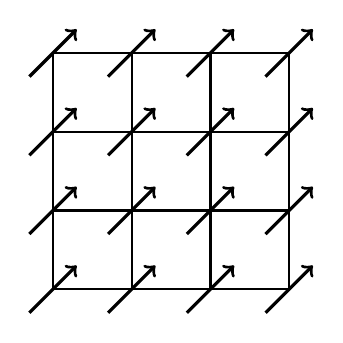
\begin{tikzpicture}
                \draw[step=1 cm, thick] (0,0) grid (3,3); %makes the grid
                \foreach \i in {0,1,2,3}{
                \foreach \j in {0,1,2,3}{
                % \node at (\i+0.05,\j) {\textcolor{cyan}{\Large \ding{218}}};
                \draw[->, very thick] (\i-0.3,\j-0.3) -- (\i+0.3,\j+0.3);
                }   
                }
                \end{tikzpicture}
                \caption{Ferromagnet}
                % \label{}
        \end{subfigure}%
        \begin{subfigure}[b]{0.5\textwidth}
                \centering
                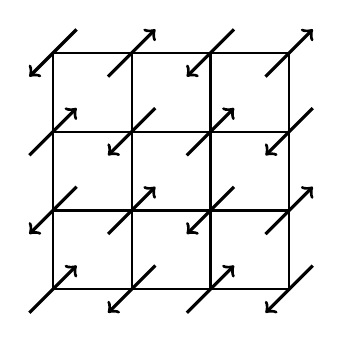
\begin{tikzpicture}
                    \draw[step=1 cm, thick] (0,0) grid (3,3);
                    \foreach \i in {0,2}
                    {
                        \foreach \j in {0,2}
                        {
                            \draw[->, very thick] (\i-0.3,\j-0.3) -- (\i+0.3,\j+0.3);
                            \draw[->, very thick] (\i+1-0.3,\j+1-0.3) -- (\i+1+0.3,\j+1+0.3);
                            \draw[->, very thick] (\i+1+0.3,\j+0.3) -- (\i+1-0.3,\j-0.3);
                            \draw[->, very thick] (\i+0.3,\j+1+0.3) -- (\i-0.3,\j+1-0.3);
                        }
                    }
                \end{tikzpicture}
                \caption{Antiferromagnet}
                % \label{}
        \end{subfigure}%
        \caption{Classical ground states on a square lattice}\label{fig:square_lattice}
\end{figure}


For the ferromagnetic case($ J < 0 $), the classical ground state would one in which all the spins are aligned in a given direction. Consider a state such that spin at each site takes the maximum value of the z component,
\begin{equation}\label{eq22}
\ket{G} = \prod_{l}^{}\ket{S}_l
\end{equation} 
The Hamiltonian will have contributions from the last term only, since the spin raising and lowering operator will destroy the state for any nearest neighbor $ <ij> $. Hence, the classical ground state is indeed the quantum ground ground state.


The classical ground state for anti-ferromagnetic case is 
\begin{equation}
	\ket{G} = \prod_{l\in A}^{}\prod_{m \in B}^{}\ket{-S}_l\ket{S}_m
\end{equation}
A and B represent the sub-lattices having spins in positive and negative z-direction respectively. Contrary to the ferromagnetic case, one of the ladder operator terms will give non-zero contribution to the classical ground state energy. This is not even an eigenstate of the Hamiltonian, let alone the ground state. To find the true ground state of a anti-ferromagnet it should be noted that it must be some sort of deviation from the classical ground state.

\section{Holstein-Primakoff Bosons}

Spin wave theory is formulated to find the quantum fluctuations around the classical ground state and in the particular case of the antiferromagnet, we can find the true ground state. 

Diagonalizing the Hamiltonian expressed in terms of the spin operators is a difficult task , given that we are only interested in the low-temperature excitation from the ground state. We seek to transform the spin operators to another set of operators such the low-lying excitation are captured as small deviations from the ground state. Towards that end, we use the Holstein-Primakoff transformation which map our system of spins to bosons. For a ferromagnet the transformation takes the following form:
\begin{equation}
\begin{split}
S^+_j &= \sqrt{2s - n_j}a_j\\
S^-_j &= a^\dagger_j\sqrt{2s - n_j}\\
S^z_j &= s - n_j
\end{split}
\end{equation}
Note that for a state with maximum projection along z-axis at site 'j', the number operator is zero. If the projection is reduced by a unit of $ \hbar $, the number operator is 1. This observation captures the idea of HP transformation: stepping down of the spin along z-axis results in creation of a boson at site j. Since the z-projection(eigenvalues of $ \mathrm{S_z} $) ranges from $\mathrm{S}$ to $\mathrm{-S}$ we have:
\begin{equation}
\expval{n_j} \leq 2s
\end{equation}
Intuitively, low-lying excitations are small collective oscillations around the ordered direction, the z-direction in our case. These oscillations make $ \expval{S_z} $ less than the maximum value s. In terms of HP representation this means that the boson number is non-zero. Since the deviations are small, the square root expansion is kept to leading orders only(known as \textit{spin wave} approximation) :
\begin{equation}
\begin{split}
S^+_j &\simeq \sqrt{2s}a_j\\
S^-_j &\simeq \sqrt{2s}a^\dagger_j\\
S^z_j &\simeq s - n_j
\end{split}
\end{equation}
In an antiferromagnet, the ordered state as two directions. If we are to use the spin-wave approximation, we have define HP transformation for the two sub-lattices. On A sub-lattice the spin projection is $ \mathrm{+S} $ so we use the previous set of transformation defined for a ferromagnet:
\begin{equation}\label{eq27}
\begin{split}
S^+_{jA} &\simeq \sqrt{2s}a_j\\
S^-_{jA} &\simeq \sqrt{2s}a^\dagger_j\\
S^z_{jA} &\simeq s - n_{jA}
\end{split}
\end{equation}
On sub-lattice B, where the spin projection is $ \mathrm{-S} $, must modify the transformation equation in the following way:
\begin{equation}\label{eq28}
\begin{split}
S^+_{Bm} &\simeq b_m^\dagger\sqrt{2s}\\
S^-_{Bm} &\simeq  \sqrt{2s}b_m\\
S^z_{Bm} &= -s + n_{mB}
\end{split}
\end{equation}

We see that depending on the number of sub-lattices, we will have to define the requisite types of transformations. If the Hamiltonian is modified and the summation index rearranged, we can get by using a single type of transformation, the ferromagnetic kind. The idea is : for each sub-lattice, for whatever spin configuration, we define a local orthonormal coordinate system such that the transformed z-axis points along the classical spin vector. Doing this we have limited the types of transformation to just the ferromagnetic type, labeled by the lattice and sub-lattice indices. 

\section{The General Spin-Wave Hamiltonian}

We develop our formalism in order to accommodate any general lattice structure. Towards that end, we need two indexes to identify a unique point in our lattice: Bravais lattice index and the corresponding sub-lattice index. To use the spin wave approximation, we will be expressing the spin operators at each site in terms of the local coordinate axes. 

The general form of the Hamiltonian describing the spin systems we wish to study is
\begin{equation}
\mathcal{H} = \frac{1}{2}\left[ \sum_{i\alpha,j\beta}^{}J\vec{S}_{i\alpha}.\vec{S}_{j\beta} + J(\Delta - 1)S_{i\alpha}^zS_{j\beta}^z  + \vec{D}_{\alpha \beta} . (\vec{S}_{i\alpha} \cross \vec{S}_{j\beta}) \right]
\end{equation}
where $\Delta$ is the anisotropy along \textit{z}-axis and $\vec{D}_{\alpha \beta}$ is Dzyaloshinski-Moriya Interaction vector between sub-lattices $\alpha$ abd $\beta$.

\noindent The spin vector operators defined in terms of the \textit{local axes}
\begin{equation}
\vec{S}_{i\alpha} = \sum_{m}^{}S^m_{i\alpha}\vec{e}^\alpha_m \quad;\quad \vec{S}_{j\beta} = \sum_{n}^{}S^n_{j\beta}\vec{e}^\beta_n
\end{equation}
Substituting above expression in Eq-2.10
\begin{equation}\label{eq31}
\mathcal{H} = \frac{1}{2}\sum_{m,n}^{}\sum_{i\alpha,j\beta}^{}D^{\alpha \beta}_{ij}(m,n)S^m_{i\alpha}S^n_{j\beta}
\end{equation}
where
\begin{equation}
    D^{\alpha \beta}_{ij}(m,n) = J\vec{e}^\alpha_m.\vec{e}^\beta_n + J(\Delta - 1)\vec{e}^\alpha_m.\hat{z}\vec{e}^\beta_n.\hat{z}   + \vec{D}_{\alpha \beta}.(\vec{e}^\alpha_m \cross \vec{e}^\beta_n)
\end{equation}
In these expressions $ e^\alpha_{m} $ are the local axes expressed in standard Cartesian system; $ \alpha $ runs over the sub-lattice index and m = x,y,z. Since the dot products are not necessarily between orthogonal unit vectors, there will be cross terms like xy,yz etc. The full Hamiltonian expanded is :
\begin{equation}
\begin{split}
\mathcal{H} = \frac{1}{2} \sum_{i\alpha j\beta}^{}  &D^{\alpha \beta}_{ij}(x,x)S^x_{i\alpha}S^x_{j\beta} + D^{\alpha \beta}_{ij}(x,y)S^x_{i\alpha}S^y_{j\beta} + D^{\alpha \beta}_{ij}(x,z)S^x_{i\alpha}S^z_{j\beta}\\ + &D^{\alpha \beta}_{ij}(y,x)S^y_{i\alpha}S^x_{j\beta} + D^{\alpha \beta}_{ij}(y,y)S^y_{i\alpha}S^y_{j\beta} + D^{\alpha \beta}_{ij}(y,z)S^y_{i\alpha}S^z_{j\beta}\\ + &D^{\alpha \beta}_{ij}(z,x)S^z_{i\alpha}S^x_{j\beta} + D^{\alpha \beta}_{ij}(z,y)S^z_{i\alpha}S^y_{j\beta} + D^{\alpha \beta}_{ij}(z,z)S^z_{i\alpha}S^z_{j\beta}  
\end{split}			
\end{equation} 
In terms of spin raising and lowering operators
\begin{equation}
\begin{split}
\mathcal{H} = \frac{1}{2}\sum_{i\alpha j\beta}^{}&J^{++}_{i\alpha j\beta}S^{+}_{i\alpha}S^{+}_{j\beta} + J^{--}_{i\alpha j\beta}S^{-}_{i\alpha}S^{-}_{j\beta} + J^{+-}_{i\alpha j\beta}S^{+}_{i\alpha}S^{-}_{j\beta}\\ + &J^{-+}_{i\alpha j\beta}S^{-}_{i\alpha}S^{+}_{j\beta} + J^{+z}_{i\alpha j\beta}S^{+}_{i\alpha}S^{z}_{j\beta} + J^{-z}_{i\alpha j\beta}S^{-}_{i\alpha}S^{z}_{j\beta}\\ + &J^{z+}_{i\alpha 
	j\beta}S^{z}_{i\alpha}S^{+}_{j\beta} + J^{z-}_{i\alpha
	j\beta}S^{z}_{i\alpha}S^{-}_{j\beta} + J^{zz}_{i\alpha\
	j\beta}S^{z}_{i\alpha}S^{z}_{j\beta}			
\end{split}
\end{equation}
The coefficients are :
\begin{equation}
\begin{split}
&J^{++}_{i\alpha j\beta} = \frac{1}{8}\left[D^{\alpha \beta}_{ij}(x,x) - D^{\alpha \beta}_{ij}(y,y) - iD^{\alpha \beta}_{ij}(x,y) - iD^{\alpha \beta}_{ij}(y,x) \right]\\
&J^{--}_{i\alpha j\beta} = \frac{1}{8}\left[ D^{\alpha \beta}_{ij}(x,x) - D^{\alpha \beta}_{ij}(y,y) + iD^{\alpha \beta}_{ij}(x,y) + iD^{\alpha \beta}_{ij}(y,x) \right]\\
&J^{+-}_{i\alpha j\beta} = \frac{1}{8} \left[ D^{\alpha \beta}_{ij} (x,x) + D^{\alpha \beta}_{ij}(y,y) + iD^{\alpha \beta}_{ij}(x,y)-iD^{\alpha \beta}_{ij}(y,x) \right]\\
&J^{-+}_{i\alpha j\beta} =\frac{1}{8} \left[ D^{\alpha \beta}_{ij} (x,x) + D^{\alpha \beta}_{ij}(y,y) - iD^{\alpha \beta}_{ij}(x,y)+iD^{\alpha \beta}_{ij}(y,x) \right]\\
&J^{+z}_{i\alpha j\beta} = \frac{1}{4}( D^{\alpha \beta}_{ij}( x,z ) - iD^{\alpha \beta}_{ij}(y,z) )\\
&J^{-z}_{i\alpha j\beta} = \frac{1}{4}( D^{\alpha \beta}_{ij}( x,z ) + iD^{\alpha \beta}_{ij}(y,z) )\\
&J^{z+}_{i\alpha j\beta} = \frac{1}{4}( D^{\alpha \beta}_{ij}( x,z ) - iD^{\alpha \beta}_{ij}(y,z) )\\
&J^{z-}_{i\alpha j\beta} = \frac{1}{4}( D^{\alpha \beta}_{ij}( z,x ) + iD^{\alpha \beta}_{ij}(z,y) )\\
&J^{zz}_{i\alpha j\beta} = \frac{1}{2}D^{\alpha \beta}_{ij}(z,z) 			
\end{split}
\end{equation}
We now replace these operators using the spin-wave approximation as follows:
\begin{equation}
\begin{split}
&S^{+}_{i\alpha} = \sqrt{2s}b_{i\alpha}\\
&S^{-}_{i\alpha} = \sqrt{2s}b_{i\alpha}^\dagger\\
&S^{z}_{i\alpha} = s - b_{i\alpha}^\dagger b_{i\alpha}
\end{split}
\end{equation}
The Hamiltonian will contain terms of different orders with respect to the boson operators. The constant term will come from $ zz $ term, order one term having a single boson operator from $ +z $,$ z+ $,$ -z $ and $ z- $ and bilinear which we would like derive explicitly. The expanded $ zz $ term,$ J^{zz}_{i\alpha j\beta}S^z_{i\alpha}S^z_{j\beta} $ looks like:
\begin{equation}
\begin{split}
&J^{zz}_{i\alpha j\beta}S^z_{i\alpha}S^z_{j\beta} \\
&= J^{zz}_{i\alpha j\beta}(s - n_{i\alpha})( s - n_{j\beta} )\\
&=J^{zz}_{i\alpha j\beta}s^2 - sJ^{zz}_{i\alpha j\beta}(n_{i\alpha} + n_{j\beta}) + J^{zz}_{i\alpha j\beta}n_{i\alpha}n_{j\beta}
\end{split}
\end{equation}
The constant term of the Hamiltonian is $ \sum_{i\alpha j\beta}^{}J^{zz}_{i\alpha j\beta}s^2 $.\\
Single operator terms come from the following:
\begin{equation}
J^{+z}_{i\alpha j\beta}s^{+}_{i\alpha}s^{z}_{j\beta} + J^{-z}_{i\alpha j\beta}s^{-}_{i\alpha}s^{z}_{j\beta} + J^{z+}_{i\alpha j\beta}s^{z}_{i\alpha}s^{+}_{j\beta} + J^{z-}_{i\alpha j\beta}s^{z}_{i\alpha}s^{-}_{j\beta}
\end{equation}
Writing the bosonic expression for the operators, :
\begin{equation}
\begin{split}			
&\sqrt{2s}J^{+z}_{i\alpha j\beta}b_{i\alpha}(s-n_{j\beta}) + \sqrt{2s}J^{-z}_{i\alpha j\beta}b_{i\alpha}^\dagger(s - n_{j\beta})\\
&\sqrt{2s}J^{z+}_{i\alpha j\beta}(s - n_{i\alpha})b_{j\beta} + \sqrt{2s}J^{+-}_{i\alpha j\beta}(s - n_{i\alpha})b_{j\beta}^\dagger
\end{split}
\end{equation}
Consider the single operator term that comes from the the previous expression and then proceed to write the lattice fourier transform for that operator.
\begin{equation}
\begin{split}
\sum_{i\alpha j\beta}^{}J^{+z}_{i\alpha,j\beta}b_{i\alpha}&\\
& = \frac{1}{\sqrt{N}} \sum_{q}^{}\sum_{i\alpha,j\beta}^{}J^{+z}_{i\alpha,j\beta}b_{q\alpha}e^{i\vec{q}.\vec{R}_i}\\
& = \frac{1}{\sqrt{N}}\sum_{q}^{}\sum_{i\alpha;j\beta}^{}J^{+z}_{i\alpha,j\beta}e^{i\frac{q}{2}.(2R_{ij} + r_{ij})}b_{q\alpha}\\
& = \sqrt{N}\sum_{\alpha}^{}(\sum_{\beta}^{}J^{+z}_{\alpha \beta}(q=0))b_{0\alpha}
\end{split}
\end{equation}
Here, indexes i and j label the bravais lattice points and $ R_{ij} = \frac{R_i + R_j}{2} \quad r_{ij} = R_i - R_j$, $ R_i $ is the position vector of the ith Bravais lattice point in the real space. Since we want the linear terms to vanish, the four coefficients must independently be zero. Thus we have :
\begin{equation}
\begin{split}
&\sum_{\beta}^{}J^{+z}_{\alpha \beta}(q = 0) = 0 \quad \sum_{\beta}^{}J^{-z}_{\alpha \beta}(q = 0) = 0\\
&\sum_{\alpha}^{}J^{z+}_{\alpha \beta}(q = 0) = 0 \quad \sum_{\alpha}^{}J^{z-}_{\alpha \beta}(q = 0) = 0
\end{split}
\end{equation}
Bilinear terms of the form $ b_{i\alpha}b_{j\beta} $ will come from $ \sum_{i\alpha;j\beta}^{}J^{++}_{i\alpha;j\beta}S^+_{i\alpha}S^+_{j\beta} $. Expanding and taking the Fourier transform we get:
\begin{equation}
\begin{split}
\sum_{i\alpha;j\beta}^{}J^{++}_{i\alpha;j\beta}S^+_{i\alpha}S^+_{j\beta}&\\
&=2s\sum_{i\alpha;j\beta}^{}J^{++}_{i\alpha;j\beta}b_{i\alpha}b_{j\beta}\\
&=\frac{2s}{N}\sum_{i\alpha,j\beta}^{}\sum_{q_1,q_2}^{}J^{++}_{i\alpha;j\beta}b_{q_1\alpha}b_{q_2\beta}e^{i(q_1.R_i + q_2.R_j)}\\
& = =\frac{2s}{N}\sum_{i\alpha,\delta \beta}^{}\sum_{q_1,q_2}^{}J^{++}_{i\alpha;j\beta}b_{q_1\alpha}b_{q_2\beta}e^{i(q_1 + q_2).R_i}e^{iq_2.\delta}\\
& = 2s\sum_{q_1,q_2}^{}\sum_{\alpha \beta}^{}\sum_{\delta}^{}J^{++}_{\alpha \beta}e^{iq_2.\delta}\delta_{q_1+q_2,0}b_{q_1\alpha}b_{q_2\beta}\\
& = 2s\sum_{q}^{}\sum_{\alpha,\beta}^{}J^{++}_{\alpha;\beta}(-q)b_{q\alpha}b_{-q\beta}
\end{split}
\end{equation}
The complex conjugate of this term will give bilinear terms of the form $ b_{i\alpha}^\dagger b_{j\beta}^\dagger $.\\Now we look at bilinear term of the form $ b_{i\alpha}^\dagger b_{j\beta} $. This comes from two sources: (i) $ J^{+-}_{i\alpha;j\beta}S^+_{i\alpha}S^-_{j\beta} + h.c $ and (ii) $J^{zz}_{i\alpha j\beta}S^z_{i\alpha}S^z_{j\beta}$. Looking at source (i):
\begin{equation}
\begin{split}
\sum_{i\alpha;j\beta}^{}J^{+-}_{i\alpha;j\beta}S^+_{i\alpha}S^-_{j\beta}&\\
&=2s\sum_{i\alpha;j\beta}^{}J^{+-}_{i\alpha;j\beta}b_{i\alpha}b^\dagger_{j\beta}\\
&=\frac{2s}{N}\sum_{i\alpha,j\beta}^{}\sum_{q_1,q_2}^{}J^{+-}_{i\alpha;j\beta}b_{q_1\alpha}b^\dagger_{q_2\beta}e^{i(q_1.R_i - q_2.R_j)}\\
& = =\frac{2s}{N}\sum_{i\alpha,\delta \beta}^{}\sum_{q_1,q_2}^{}J^{+-}_{i\alpha;j\beta}b_{q_1\alpha}b^\dagger_{q_2\beta}e^{i(q_1 - q_2).R_i}e^{-iq_2.\delta}\\
& = 2s\sum_{q_1,q_2}^{}\sum_{\alpha \beta}^{}\sum_{\delta}^{}J^{+-}_{\alpha \beta}e^{-iq_2.\delta}\delta_{q_1-q_2,0}b_{q_1\alpha}b^\dagger_{q_2\beta}\\
&=2s\sum_{q}^{}\sum_{\alpha,\beta}^{}J^{+-}_{\alpha;\beta}(-q)b_{q\alpha}b^\dagger_{q\beta}
\end{split}
\end{equation}
Adding the hermitian conjugate of the above to itself (exchange the role of the indexes since they run independently over all the sub-lattice points):
\begin{equation}
\begin{split}
\sum_{i\alpha;j\beta}^{}J^{+-}_{i\alpha;j\beta}S^+_{i\alpha}S^-_{j\beta}&\\
&=2s\sum_{q}^{}\sum_{\alpha \beta}^{}[J^{+-}_{\beta \alpha}(-q) + (J^{+-}_{\alpha \beta}(-q))^*]b_{q\alpha}^\dagger b_{q\beta}
\end{split}
\end{equation}
Now we look at the source (ii), the bilinear terms are:
\begin{equation}
\begin{split}
&-s\sum_{i\alpha;j\beta}^{}J^{zz}_{i\alpha;j\beta}(b^\dagger_{i\alpha}b_{i\alpha} + b^\dagger_{j\beta}b_{j\beta})\\
&=-s\sum_{q;\alpha;\beta}^{}J^{zz}_{\alpha;\beta}(0)(b^\dagger_{q\alpha}b_{q\alpha} + b^\dagger_{q\beta}b_{q\beta})\\
&=-s\sum_{q;\alpha;\beta}^{}(J^{zz}_{\alpha;\beta}(0) + J^{zz}_{\beta;\alpha}(0))b^\dagger_{q\alpha}b_{q\alpha}
\end{split}
\end{equation}

So the full spin-wave Hamiltonian is :
\begin{equation}
\begin{split}
\mathcal{H} = &\sum_{i\alpha;j}^{}J^{zz}_{i\alpha;j\beta}s^2\\
&+2s\sum_{q}^{}\sum_{\alpha,\beta}^{}J^{++}_{\beta,\alpha}(-q)b_{-q\alpha}b_{q\beta}\\
&+2s\sum_{q}^{}\sum_{\alpha,\beta}^{}(J_{\alpha,\beta}^{++}(-q))^*b^\dagger_{q\alpha}b^\dagger_{-q\alpha}\\
&+2s[\sum_{q}^{}\sum_{\alpha,\beta}^{}(J^{+-}_{\beta,\alpha}(-q) + (J^{+-}_{\alpha,\beta}(-q))^*) + \frac{1}{2}\delta_{\alpha,\beta}(\sum_{\gamma}^{}J^{zz}_{\alpha,\gamma}(0) + J^{zz}_{\gamma,\alpha}(0)) ]b^\dagger_{q\alpha}b_{q\beta}
\end{split}
\end{equation}
Using the commutation relation for the boson operators and expressing the Hamiltonian as $ \sum_{full-zone}^{}H(q) = \sum_{half-zone}^{}(H(q) + H(-q)) $ we get
\begin{equation}
	\begin{split}
		\mathcal{H}_{spinwave} &= \sum_{i\alpha,j\beta}^{}J^{zz}_{i\alpha,j\beta}s^2\\
		&-2s\sum_{q}^{}\sum_{\alpha}^{}(J^{+-}_{\alpha \alpha}(q) + (J^{+-}_{\alpha \alpha}(q))^* )\\
		&-s\sum_{\alpha}^{}\left( \sum_{\gamma}^{} (J^{zz}_{\alpha \gamma}(0) + J^{zz}_{\gamma \alpha}) \right)\\
		&+2s\sum_{q}^{}\sum_{\alpha,\beta}^{}\left(J^{++}_{\beta,\alpha}(-q) + J^{++}_{\alpha, \beta}(q) \right)b_{-q\alpha}b_{q\beta}\\
		&+2s\sum_{q}^{}\sum_{\alpha,\beta}^{}\left((J_{\alpha,\beta}^{++}(-q))^* + (J_{\beta,\alpha}^{++}(q))^* \right)b^\dagger_{q\alpha}b^\dagger_{-q\alpha}\\
		&+2s[\sum_{q}^{}\sum_{\alpha,\beta}^{}(J^{+-}_{\beta,\alpha}(-q) + (J^{+-}_{\alpha,\beta}(-q))^*) - \frac{1}{2}\delta_{\alpha,\beta}(\sum_{\gamma}^{}J^{zz}_{\alpha,\gamma}(0) + J^{zz}_{\gamma,\alpha}(0)) ]b^\dagger_{q\alpha}b_{q\beta}\\
		&+2s[\sum_{q}^{}\sum_{\alpha,\beta}^{}(J^{+-}_{\beta,\alpha}(q) + (J^{+-}_{\alpha,\beta}(q))^*) - \frac{1}{2}\delta_{\alpha,\beta}(\sum_{\gamma}^{}J^{zz}_{\alpha,\gamma}(0) + J^{zz}_{\gamma,\alpha}(0)) ]b_{-q\alpha}b^\dagger_{-q\beta}
	\end{split}
\end{equation}
In order to diagonalize the Hamiltonian, we recast the bilinear terms in the following form:
\begin{equation}
	\mathcal{H} = \textbf{a}^\dagger\mathcal{D}\textbf{a}
\end{equation}
where $ \mathcal{D} $ is called the dynamical matrix with dimensions twice the number of sub-lattices.

 \[
 \mathcal{D} =
\left[ {\begin{array}{cc}
	\Delta _1 & \Delta _2 \\
	\Delta _3 & \Delta _4 \\
	\end{array} } \right]
\]
The corresponding matrix elements of the general bi-linear Hamiltonian are:
\begin{equation}
	\begin{split}
		&(\Delta _1)_{\alpha \beta} = (J^{+-}_{\beta,\alpha}(-q) + (J^{+-}_{\alpha,\beta}(-q))^*) - \frac{1}{2}\delta_{\alpha,\beta}(\sum_{\gamma}^{}J^{zz}_{\alpha,\gamma}(0) + J^{zz}_{\gamma,\alpha}(0)) \\
		&(\Delta _2)_{\alpha \beta} = (J_{\alpha,\beta}^{++}(-q))^* + (J_{\beta,\alpha}^{++}(q))^*\\
		&(\Delta _3)_{\alpha \beta} = J^{++}_{\beta,\alpha}(-q) + J^{++}_{\alpha, \beta}(q)\\
		&(\Delta _4)_{\alpha \beta} = J^{+-}_{\beta,\alpha}(q) + (J^{+-}_{\alpha,\beta}(q))^*) - \frac{1}{2}\delta_{\alpha,\beta}(\sum_{\gamma}^{}J^{zz}_{\alpha,\gamma}(0) + J^{zz}_{\gamma,\alpha}(0))
	\end{split}	
\end{equation}

\section{Diagonalisation}
Diagonalisation of the hamiltonian of the form 
\begin{equation}
    \mathcal{H} = \textbf{a}^\dagger\mathcal{D}\textbf{a}
\end{equation}
amounts to finding a transformation $\mathcal{T}$
\begin{equation}
\begin{split}
       \begin{pmatrix}
        \gamma ^\dagger \quad \gamma
    \end{pmatrix}
     &= \begin{pmatrix}
     \alpha ^\dagger \quad \alpha
     \end{pmatrix}
     \mathcal{T}^\dagger \\
     \begin{pmatrix}
        \gamma  \\ \quad \gamma ^\dagger
    \end{pmatrix}
     &= \mathcal{T}\begin{pmatrix}
     \alpha \\ \quad \alpha ^\dagger
     \end{pmatrix}
\end{split}
\end{equation}
which will render the spin wave Hamiltonian to be diagonal
\begin{equation}
    \mathrm{H} = \textbf{a}^\dagger\mathcal{D}\textbf{a} = \textbf{a}^\dagger\mathcal{T}^\dagger(\mathcal{T}^\dagger)^{-1}\mathcal{D}\mathcal{T}^{-1}\mathcal{T}\textbf{a}
\end{equation}
The eigenvalues are given by
\begin{equation}
    (\mathcal{T}^\dagger)^{-1}\mathcal{D}\mathcal{T}^{-1} = \mathcal{E}
\end{equation}
The algorithm to find the transformation matrix:
\begin{itemize}
		\item Generate the dynamical matrix for each wavevector, $ q $
		\item Using Cholesky decomposition, find $ \mathcal{K} $ such that $ \mathcal{D} = K^\dagger K $
		\item Do a unitary diagonalization of $ KIK^\dagger $, where I is the para-unit matrix
		\item The transformation matrix $\mathcal{T} = K^{-1}U\mathcal{E}^{\frac{1}{2}}$, where $U$ is the unitary matrix digonalising $KIK^\dagger$. 
\end{itemize}
\setcounter{equation}{0}
\setcounter{table}{0}
\setcounter{figure}{0}
%\baselineskip 24pt


    



